\section{Applications}\label{sec-application}

\begin{figure*}[h]
    \centering
        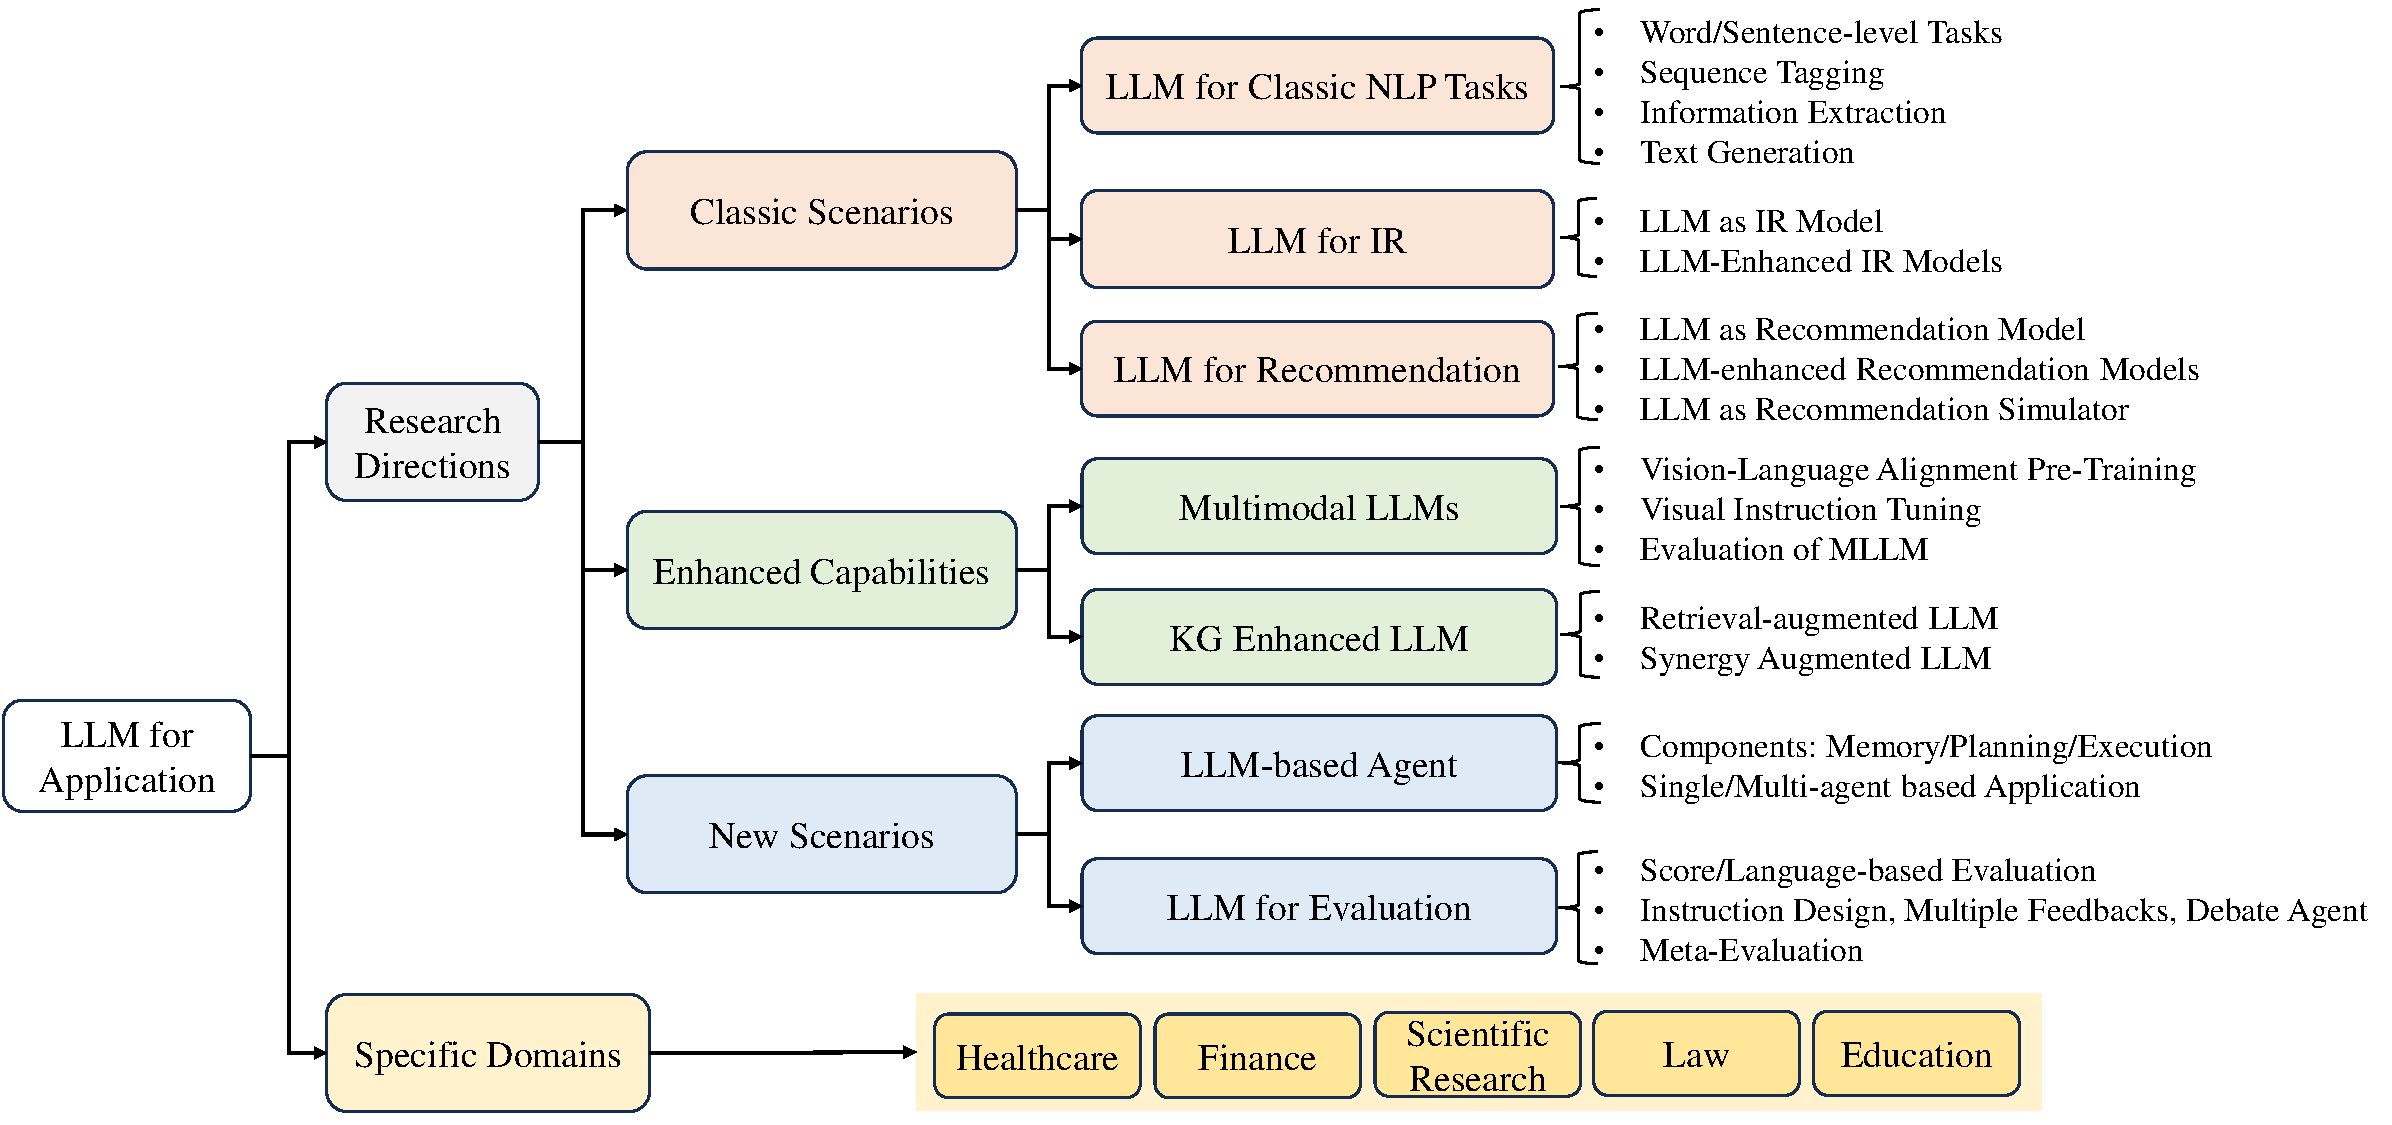
\includegraphics[width=1\textwidth]{images/application.pdf}
    \caption{The applications of LLMs in representative research directions and downstream domains. }
    \label{fig:application}
\end{figure*}

{In this section, we briefly review the recent progress on the applications of LLMs in two aspects, namely the impact to research community and representative domains.}
Figure~\ref{fig:application} shows a content organization of this section\footnote{Note that we don't aim to cover all the related research directions or domains, but instead demonstrating the use or impact of LLMs via these selected examples. }. 

\subsection{LLM for Research Community} \label{sec:llm4community}
As LLMs have revolutionized the way how we develop AI algorithms, it poses significant impact on the research community. In this part, we briefly review the advances that led by LLMs for  several representative research directions.  


\subsubsection{LLM for Classic NLP Tasks}
As pre-trained language models (\eg BERT) have originated in the field of NLP, the technical advances of language models has an important impact on the research of NLP. In this part, we discuss the application of LLMs on five kinds of classic NLP tasks, including word-level, sentence-level, sequence tagging, relation extraction, and text generation tasks, which had been the foundation of many existing NLP systems and applications.   
Note that we do not intend to comprehensively cover all NLP tasks, but instead try to analyze the impact of LLMs for fundamental NLP research through the basic tasks.
We also omit the discussion of several tasks (\eg language modeling) that have been discussed early in this survey. 


\paratitle{Word/Sentence-level Tasks.}
As long-standing NLP tasks, word-level (\eg word clustering~\cite{Martin-Speech-1998-clustering} and sense disambiguation~\cite{Navigli-ACM-2009-disambiguation}) and sentence-level tasks (sentence matching~\cite{Gomaa-International-2013-similarity} and sentiment classification~\cite{Minaee-ACM-2021-classification}) have been widely studied in the literature and applied in real-world platforms. 
To solve these tasks, the key is to accurately understand the semantic information about the words or sentences.
As rich high-quality labeled data about these tasks has been accumulated so far, existing work~\cite{qiu-CoRR-2020-PTM,Devlin-NAACL-2019-BERT} finds that small language models can achieve very good performance by fine-tuning on it.
Recent studies~\cite{Brown-NeurIPS-2020-Language,Alex-NIPS-2021-RAFT} have also tested the performance of LLMs on these tasks, showing that LLMs can also perform well via in-context learning (with very few examples).   
Whereas,  {as small models can be specially optimized on these tasks to learn the specific task requirement  and domain knowledge}, full-data fine-tuned small models can mostly outperform LLMs using in-context learning on several classic tasks~\cite{Qin-arxiv-2023-Is,Chen-arxiv-2023-Robust}, \eg semantic matching and sentiment analysis. 



\paratitle{Sequence Tagging.}
The sequence tagging tasks, \eg named entity recognition~(NER)~\cite{Nadeau-Lingvisticae-2007-NER} and part-of-speech~(POS) tagging~\cite{Ratnaparkhi-EMNLP-1996-maximum}, are also fundamental tasks. 
Typically, such tasks require assigning each token in the input sequence a proper semantic category label, \eg the classic B-I-O (\emph{Beginning}, \emph{Inside} and \emph{Outside}) tagging scheme for NER tasks.
In the era of deep learning, early efforts~\cite{Yadav-COLING-2018-survey,Souza-arxiv-2019-portuguese} mainly integrate the learned sequence representations (\eg using CNN, LSTM, and BERT) into the classic conditional random field model~(CRF), which performs the tagging task based on structural  prediction.
Recently, researchers have tested the performance of  LLMs in sequence tagging tasks, but observed that LLMs still face challenges in solving them using in-context learning~\cite{Qin-arxiv-2023-Is}, especially for special categories with ambiguous or rare names, \eg the ``MISC'' (\emph{miscellaneous entity}) and ``ORG'' (\emph{organization}) classes.
A possible reason is that LLMs may misunderstand the meanings of these classes in the human-annotated dataset, making it difficult to accurately  understand their semantics according to the instruction and limited examples in the context.


\paratitle{Information Extraction.}
The information extraction task focuses on automatically extracting useful structured information from unstructured text data, such as relation extraction~\cite{Pawar-arxiv-2017-relation} and event extraction~\cite{walker-ldc-2006-ace}, which is also a crucial task relating to many NLP applications.
Typically, previous studies formulate this task as a text classification task or a sequential labeling task.
{As information extraction often needs to accurately understand and process complex semantic relations  (multiple relations within one sentence),  in-context learning with LLMs typically underperform state-of-the-art full-data fine-tuning methods~\cite{gao-arxiv-2023-exploring,ma-arxiv-2023-Large}.}
Whereas, it is shown that enabling collaboration between LLMs and small models can further boost the performance of specific tasks~\cite{tang-arxiv-2023-does,ma-arxiv-2023-Large}. 
In addition, a recent study~\cite{wei-arxiv-2023-zero} also reveals that LLMs can achieve competitive zero-shot performance for information extraction with a two-stage workflow, making this approach attractive in future applications.


\paratitle{Text Generation.}
{Text generation tasks, \eg machine translation~\cite{Bahdanau-ICLR-2015-Neural} and automatic summarization~\cite{Nallapati-acl-2016-Abstractive}, are long-standing NLP tasks that have been widely studied, and there have been a number of deployed products and systems based on fine-tuned small models~\cite{Wu-arxiv-2016-Google,vaswani-CAMT-2018-tensor2tensor}.
Since the pre-training of LLMs is established on text prediction, they exhibit strong language generation abilities  as commercial products~\cite{Jiao-arxiv-2023-mt} and humans~\cite{Zhang-2023-arxiv-Benchmarking}, with the help of proper prompts~\cite{zhang-arxiv-2023-prompting,ghazvininejad-arxiv-2023-dictionary}. 
Additionally, LLMs are flexible to effectively handle special requirement in real-world application scenarios, \eg document-level translation~\cite{wang-arxiv-2023-document}, and also enable natural language interaction with users to further improve the generation quality~\cite{jiao-arxiv-2023-parrot}.
Despite the above success, recent work also reveals that LLMs are hard to well address the generation tasks about low-resource languages and domains, \eg Marathi-to-English translation~\cite{yang-arxiv-2023-bigtrans}, due to their unbalanced training data across different languages.
}


\paratitle{Summary}. 
{Based on the above discussion, we summarize the suggestions, and future direction about the use of LLMs in classic NLP tasks as follows:}

$\bullet$ \emph{Suggestions:}
LLMs and small models have their own merits in different aspects: LLMs are can provide unified solutions to various NLP tasks and achieve competitive performance (especially in the zero/few-shot setting), while small models are economical to develop and can be specially tuned according to target tasks, which can achieve good performance with sufficient high-quality labeled data~\cite{Qin-arxiv-2023-Is,Chen-arxiv-2023-Robust,Kocon-arxiv-2023-ChatGPT,Zhong-arxiv-2023-Can}.  
In applications, one can make suitable choices based on the actual needs, comprehensively considering flexibility, data availability, training compute, and efficiency.


$\bullet$ \emph{Future direction:} 
{%
{Despite the excellent general capacities, LLMs still cannot effectively process the NLP tasks in low-resource domains, \eg minor language translation. 
To tackle such tasks, it needs to develop effective approaches to injecting necessary task information or domain-specific knowledge into LLMs, either through fine-tuning or prompting. %
In addition, it is still challenging for LLMs to handle complex semantic relations in classic NLP tasks (\eg nested entity extraction), which is worth more exploration from the underlying working mechanism of LLMs. 
}
It is also promising to combine LLMs and fine-tuned small language models for complementing with each other in solving complex cases of classic NLP tasks~\cite{Cheng-arxiv-2023-UPRISE}. 
Another promising direction is to conduct human-machine collaborative research (\eg conversational translation~\cite{jiao-arxiv-2023-parrot}) on NLP tasks, since LLMs can effectively understand human instructions and make meaningful responses. 
}

\subsubsection{LLM for Information Retrieval}
{
The goal of information retrieval~(IR) systems is to assist users in discovering ideal information resources~(typically documents) and mitigating the information overload issue.
Typically, contemporary IR systems adopt a  retrieve-then-rerank pipeline framework~\cite{Zhao-arxiv-2022-Dense}. Within this framework, the retriever initially retrieves relevant information from a large-scale corpus, and the reranker subsequently performs multi-stage  ranking procedure to acquire the most relevant information~\cite{Ren-EMNLP-2021-rocketqav2}.
Since the advent of LLMs has significant impact on the way of information access, we discuss how it advances the development of IR from two main aspects, namely LLMs as IR models and LLM-enhanced IR models.   
}

\paratitle{LLMs as IR Models.}
{Existing IR models can be overall categorized into \emph{sparse models} (relying on term-based lexical similarity) and \emph{dense models} (relying on embedding based semantic similarity)~\cite{Zhao-arxiv-2022-Calibrating}.  Specially, dense models are mainly implemented by fine-tuned PLMs (\eg BERT).   
Compared to PLMs, LLMs have more strong model capacities in capturing text semantics, thus having the potential to improve existing dense IR models. 
However, due to the high overhead of LLMs, %
the majority of studies concentrate on employing LLMs as rerankers, aiming to refine the ranking of retrieved candidates. %
To achieve this, recent efforts often formulate special instructions that enable LLMs to perform reranking on a small set of provided candidate documents. Typically, such an approach does not necessitate model training, and achieve promising results compared with well-trained reranking methods~\cite{sun-arxiv-2023-chatgpt, qin-arxiv-2023-large}. 
Specially, the LLM-based reranking approach can be implemented in different ways by zero-shot or few-shot instruction, including  pointwise (\emph{estimating the relevance scores for query-document pairs})~\cite{Cho-ACL-2023-Discrete}, pairwise (\emph{determining the  relevance order of two documents})~\cite{qin-arxiv-2023-large}, or listwise ranking (\emph{sorting a subset of candidate documents})~\cite{tang-arxiv-2023-found}.  
{The essence of these methods lies in the special design of  instructions for text reranking, such as sliding window strategy for document lists~\cite{sun-arxiv-2023-chatgpt, ma-arxiv-2023-zero}, setwise selection prompting~\cite{zhuang-arxiv-2023-setwise}, fine-grained relevance labels incorporation~\cite{zhuang-arxiv-2023-beyond}, and pairwise comparison prompting~\cite{qin-arxiv-2023-large}.}
In addition, recent efforts employ LLMs to generate intermediate texts (\eg URLs) as retrieval results using few-shot demonstrations~\cite{ziems-arxiv-2023-large}.
To further enhance the model performance, LLMs can be specially fine-tuned as  backbones for reranking~\cite{Ma-arxiv-2023-fine, pradeep-arxiv-2023-rankvicuna} or retrieval~(including dense retrieval~\cite{Zhao-arxiv-2022-Dense} and model-based retrieval~\cite{Tay-NIPS-2022-transformer, Ren-ACL-2023-tome}), similar to the fine-tuning process for traditional PLM-based IR models~\cite{Ma-arxiv-2023-fine}. However, fine-tuning LLMs as IR models entails considerable expenses given the huge parameter scale of LLMs.
}



\paratitle{LLM-Enhanced IR Models.}
{As another major research direction, LLMs can be employed to improve existing IR models (\eg small models).  
A common challenge faced by existing IR models is the lack of relevant judgment annotation~\cite{Qu-NAACL-2021-rocketqa, Ren-ACL-2021-PAIR}. 
To tackle this problem, LLMs can be instructed to annotate positive or negative documents for a given query~\cite{peng-arxiv-2023-soft}, or to generate corresponding queries based on a set of documents in the corpus by referring to a few demonstrations~\cite{Dai-ICLR-2023-promptagator, askari-arxiv-2023-generating}.
In addition to training data augmentation, LLM has the potential to improve existing IR models by refining the search-oriented informativeness of both queries and documents.   
In IR systems, the input queries may be constrained by a user's cognitive and cultural competency, making it challenging to accurately  express the real intent, and irrelevant content  present in documents can also impact the relevance evaluation with the query.
As a solution, LLM can be utilized to rewrite the query for enhancing the understanding of the query intent and incorporating additional knowledge into the query through well-designed instructions. The rewritten query can take the form of an improved version of the original query~\cite{mao-arxiv-2023-large}, {a document in the corpus that related to the query~\cite{Gao-ACL-2023-precise}, or an expansion of the query that concatenated with a pseudo generated document~\cite{Wang-arxiv-2023-query2doc}.} 
In addition, documents can also be expanded with queries that are generated based on the original documents using LLMs for context extension~\cite{ma-arxiv-2023-pre}.}



\paratitle{Remaining Issues.} 
{
In this part, we further discuss several important issues to apply LLMs to improve IR  systems. 
First, though LLMs are capable of being as general-purpose task solvers, they are not directly well suited for existing IR systems: they require high overhead for inference~\cite{sun-arxiv-2023-chatgpt, Ma-arxiv-2023-fine}, have limitations in modeling long texts or document lists~\cite{ma-arxiv-2023-zero}, and need special adaptation (\eg instruction tuning) to perform the text ranking task~\cite{sun-arxiv-2023-instruction}.  
Therefore, more systematic approaches to adapt LLMs for modern IR systems should be investigated, to leverage their benefits and meanwhile overcome these limitations. 
Secondly, the advent of LLMs sheds lights on the development of new information seeking ways (\eg New Bing). 
It is meaningful to explore how to reshape the architecture and paradigm of IR by integrating the LLMs' capacities and the merits of existing IR systems~\cite{wang-arxiv-2023-large}. 
Thirdly, existing work mainly focuses on text retrieval tasks, lacking a comprehensive consideration of multimodal information sources. 
As will be discussed in Section~\ref{sec-MLLM}, multimodal large language models~\cite{Li-arXiv-2023-Multimodal} 
are also widely studied, making it feasible to develop more powerful multimedia retrieval systems. 
}




\subsubsection{LLM for Recommender Systems} 
{
Unlike IR systems that analyze user search queries to retrieve relevant documents, recommender systems (RS) aim to capture the underlying user preference and provide appropriate information resources to users~\cite{zhao-cikm-2021-recbole, zhou-cikm-2021-s3rec, Zhao-cikm-2022-recbole-2, Xu-sigir-2023-towards}. 
Typically, existing studies train a recommendation model (either classic or deep learning model) by fitting it over the user's logged data (\eg click data)~\cite{Rendle-arxiv-2012-bpr, Kang-ICDM-2018-Self}.  
However, these models often suffer from a series of technical issues, \eg cold-start recommendation, domain transfer, and poor explainability. 
Recently, LLMs have demonstrated the potential to alleviate these issues of recommendation models~\cite{Zhang-2023-arxiv-recommendation, fan-arxiv-2023-recommender, wu-arixv-2023-a}, due to the strong  capacities of domain generalization and language generation.   
In this part, we briefly
review the recent progress of LLMs in recommender systems, from the following three aspects, namely LLMs as recommendation models, LLM-enhanced recommendation models, and LLMs as recommendation simulators. 
}



\paratitle{LLMs as Recommendation Models.}
{
 With specific methods or mechanisms, LLMs can be adapted to serve as recommendation models.  
Existing work along this line can be generally divided into two main categories. First, some methods prompt LLMs for completing the recommendation task in a zero-shot paradigm (\ie without parameter tuning)~\cite{Gao-arxiv-2023-chat-rec, dai-recsys-2023-uncovering}. A series of prompt engineering methods like recency-focused and in-context learning are introduced to improve recommendation performance as well as alleviate the potential model biases~\cite{hou-arxiv-2023-large, Liu-arxiv-2023-is}.
Second, another category  of studies aim to specialize LLMs for personalized recommendation through instruction tuning~\cite{Zhang-2023-arxiv-recommendation,bao-recsys-2023-tallrec}. Specially, high-quality  instruction data is key to adapt LLMs to the recommendation tasks, which can be constructed based on user-item interactions with heuristic templates. To further improve the instruction diversity, 
InstructRec~\cite{Zhang-2023-arxiv-recommendation} employs self-instruct technique to simulate large amounts of potential user instructions in various scenarios like product search and personalized recommendations. In addition to representing each item by its text description, there is also growing attention on extending LLM's vocabulary  with semantic identifiers in recommender systems~\cite{Zhu-arxiv-2023-Collaborative,Zheng-2023-arxiv-Adapting}, to incorporate collaborative semantics into LLMs.}





\paratitle{LLM-enhanced  Recommendation Models.}
{
In addition to instructing LLMs to directly provide recommendations, researchers also propose leveraging the universal knowledge encoded in LLMs to improve traditional recommender systems. 
Existing approaches in this line can be divided into three main categories. The first category employs LLMs to infer users' potential intention from their historical interaction data. Furthermore, traditional recommendation/search models employ the inferred intentions to improve the retrieval of  relevant items~\cite{xi-arxiv-2023-towards, liu-arxiv-2023-a}. Additionally, several studies explore the use of LLMs as feature encoders. %
They employ LLMs to encode the side information of items and users (\eg item's descriptions and user's reviews), %
thus deriving more informative representations of users and items. These representations are then fed into traditional recommender systems as augmented  input~\cite{li-arxiv-2023-exploring, Wei-arixiv-2023-llmrec}. %
{
As another alternative approach, 
several studies~\cite{Li-arxiv-2023-ctrl, Muhamed-nips-2021-ctr-bert} adopt a distillation-like way to transfer LLM's    capacities (\eg semantic encoding) to improve traditional recommenders (\ie small models). 
Specially, they align the hidden states of LLMs and traditional recommendation models via joint training. After training, since only the enhanced small model will be deployed online,  it can avoid  the huge overhead of LLMs in online service.    
}



















\paratitle{LLM as Recommendation Simulator.} 
{Inspired by the recent success of autonomous AI agents~\cite{wang-arxiv-2023-a}, LLMs have been also utilized to develop recommendation simulators~\cite{Wang-arxiv-2023-RecAgent, Ie-arxiv-2019-recsim} (exemplified by RecAgent~\cite{Wang-arxiv-2023-RecAgent}), showing  great potential to simulate user real behaviors in recommender systems~\cite{Wang-arxiv-2023-RecAgent, Zhang-arxiv-2023-AgentCF, zhang-arxiv-2023-on}.   
Specifically, to make  personalized simulation, an agent will be equipped with a profiling module that encompasses relevant identity information.  Then, a memory module is introduced to store agents' past interaction experiences.  
During the process of simulation, agents are further prompted to conduct self-reflection based on their past experiences, to capture their underlying user preference.  
Most of existing recommendation simulators are conducted in a user-oriented way, without explicitly modeling the items in the interaction process.  
To address this, AgentCF~\cite{Zhang-arxiv-2023-AgentCF} models both users and items as agents,  and further facilitates collaborative reflections to simulate user-item interactions, so as to capturing the two-sided relations between users and items.}
 








\paratitle{Remaining Issues.} 
{
Despite these efforts, there are still several challenges to address when applying LLMs in recommender systems. First, existing studies have shown that LLM-based  recommendation models in zero/few-shot settings tend to perform worse than traditional ID-based recommenders~\cite{hou-arxiv-2023-large, dai-recsys-2023-uncovering}. This indicates that LLMs might lack an understanding of personalized user behaviors and domain-specific collaborative semantics. Although instruction tuning  alleviates this issue to some extent~\cite{bao-recsys-2023-tallrec, Zhang-2023-arxiv-recommendation}, it can't fully reduce the semantic gap between LLMs and recommender systems, and also suffers from high tuning costs.  
Furthermore, recommender systems prioritize minimizing inference latency to enhance users' experience in low-resourced environments (\eg phones), which poses a challenge to LLMs'  inference speed as well as memory overhead. Therefore, it is important to explore  improvement  techniques, such as efficient tuning and quantization methods, to deploy LLMs efficiently and effectively in real-world recommender systems. In addition, existing LLMs
have limited capacities in long context modeling, make it difficult to process the huge amount of user-item interaction data. Improved context length  extension and context information utilization approaches should be developed to improve the modeling capacities of LLMs in long interaction sequences. 
}









\subsubsection{Multimodal Large Language Model}\label{sec-MLLM}
{In existing literature~\cite{Du-arxiv-2023-survey,Gan-Foundation-2022-vision}, multimodal models mainly refer to the models that can process and integrate information of various  modalities (\eg text, image, and audio) from input, and further produce corresponding output in certain modalities. 
In this part, we mainly focus on the multimodal extension of LLMs by enabling the information modeling of non-textual modalities, especially the vision modality, called \emph{multimodal large language models~(MLLMs)}~\cite{Li-arXiv-2023-Multimodal}\footnote{In existing work, large vision language models~(LVLMs)~\cite{Li-arxiv-2023-Evaluating} are also used to term such bimodal models that are developed based on LLMs. We use the naming of MLLMs in this part due to its wide use in existing literature. }. 
To start our discussion, we specify the input to be text-image pairs and the output to be text responses. Similar discussions can be made for other modalities, \eg language-audio  models~\cite{Rubenstein-2023-arxiv-audiopalm}, which is beyond our scope here.  
In essence, MLLMs are developed by adapting the information from other modalities to the text modality, so as to leverage the excellent model capacities of LLMs that are learned based on world text. %
Typically, a MLLM comprises an image encoder for image encoding and a LLM for text generation, associated by a connection module that aligns vision and language representations. During generation, the image is first split into patches, and then transformed into patch embeddings by the image encoder and the connection module, to derive a visual representation that can be understood by the LLM. Subsequently, the patch embeddings and text embeddings are concatenated, and fed into the MLLM, allowing the language model to generate the response autoregressively. In the following, we will discuss the training, evaluation, and key points to develop capable MLLMs.}

\paratitle{Training Process.}
{The training process of the MLLM includes two major stages: vision-language alignment pre-training and visual instruction tuning.} 

\textbullet~\emph{Vision-language alignment pre-training.}
 {To develop MLLMs, existing work mostly initializes the vision encoder and the LLM with pre-trained models~\cite{Alayrac-nips-2022-flamingo, Liu-arxiv-2023-Visual, Zhu-arxiv-2023-MiniGPT-4}. These models retain excellent vision and language capacities, but span different semantic spaces. Thus, the goal of vision-language alignment pre-training (\ie the first-stage training) is to align the vision encoder and the LLM through end-to-end training on large-scale image-text pairs~\cite{Schuhmann-nips-2022-laion5b, Changpinyo-cvpr-2023-conceptual}. However, directly tuning these two models on image-text pairs may cause the degradation of the original representation capacities. %
 To improve the alignment performance, it is crucial to design effective training strategies and select appropriate pre-training data~\cite{Ye-arxiv-2023-mplug, Bai-arxiv-2023-qwen}.  
% 
Existing work mainly employs the following strategies for cross-modality alignment: (1) if the number of image-text pairs is not sufficiently large~(\eg less than 1M), it is often suggested to only update the connection module~\cite{Liu-arxiv-2023-improved}; (2) if the training data includes high-quality text corpora~\cite{Zhang-arxiv-2023-internlm} or image-text pairs with fine-grained annotations~\cite{Chen-arxiv-2023-shikra},  fine-tuning the LLM can be conducted to boost the performance;  (3) if the number of image-text pairs is very large~(\eg about 1B), fine-tuning the vision encoder is also plausible~\cite{Ye-arxiv-2023-mplug,Bai-arxiv-2023-qwen}, but the benefit remains further verification.} 

\textbullet~\emph{Visual instruction tuning.}  %
{After vision-language pre-training, the second-stage training, \ie visual instruction tuning, aims to improve the instruction-following and task-solving abilities of MLLMs. Generally, the input of visual instruction tuning consists of an image and a task description, and the task is to generate a corresponding text output. 
To boost the performance, high-quality visual instruction data is key to eliciting and enhancing the abilities of MLLMs. 
Therefore, most studies are dedicated to constructing various visual instruction datasets. As the basic approaches, early studies construct visual instructions by distilling from GPT-4~\cite{Liu-arxiv-2023-Visual} or reformulating vision-language task datasets~\cite{Dai-2023-arxiv-InstructBLIP}. To enhance the quality of instruction data, recent work further proposes improved strategies by increasing the instruction diversity~\cite{liu-arxiv-2023-aligning}, incorporating fine-grained information~(\eg coordinate of objects) into the instruction~\cite{Chen-arxiv-2023-shikra}, or synthesizing complex visual reasoning instructions~\cite{Du-arxiv-2023-What}.  
}

\paratitle{Evaluation of MLLM.} {After introducing the approaches to developing MLLMs, we further discuss how to effectively assess the multimodal capabilities of MLLMs from the following three aspects.  
}

\textbullet~\emph{Evaluation perspectives.} 
{The evaluation tasks for MLLMs can be categorized into two main types: \emph{perception} and \emph{cognition} tasks. Specifically, \emph{perception} tasks aim to assess the model's abilities in understanding the basic semantics of the image content, while \emph{cognition} tasks evaluate models with more complex tasks that require reasoning based on perception results. 
The perception ability is typically evaluated through classification tasks about attributes of image (\eg topic and style) and object (\eg existence and color) or OCR-related tasks, based on existing datasets or new datasets derived from existing images with annotations by humans or LLMs~\cite{Gurari-cvpr-2018-vizwiz, Mishra-cvpr-2012-top, Liu-arxiv-2023-mmbench, Fu-arxiv-2023-mme}. 
A notable perception issue is hallucination~\cite{Zhang-arxiv-2023-siren}, where the model's responses contain inconsistent content with the image. 
Among existing studies about hallucination in MLLMs~\cite{liu-arxiv-2023-aligning, Gunjal-arxiv-2023-detecting, Lu-arxiv-2023-evaluation}, object hallucination~\cite{Rohrbach-emnlp-2018-object} has received much research attention.  
To conduct a stable, robust evaluation of object hallucination, POPE~\cite{Li-emnlp-2023-evaluating} proposes a polling-based object probing approach for converting object recognition into a series of binary questions, and the results indicate that current MLLMs often struggle with object hallucination.
Cognition tasks, on the other hand, require MLLMs to perform reasoning based on image perception. A common reasoning task is visual question answering (VQA), where models answer questions about images that demand reasoning about spatial relationships~\cite{Hudson-cvpr-2019-gqa}, general knowledge~\cite{Lu-nips-2022-learn}, or scene text~\cite{Amanpreet-cvpr-2019-textvqa}. To fully explore the capabilities of MLLMs, HallusionBench~\cite{Liu-arxiv-2023-hallusionbench} collects 200 sophisticated visual dependent or supplement questions, on which even the most advanced MLLMs like LLaVA-1.5~\cite{Liu-arxiv-2023-improved} and GPT-4V~\cite{OpenAI-OpenAI-2023-GPT-4v} fail to achieve good performance.}

\textbullet~\emph{Evaluation paradigms.}{
The responses of MLLMs can be evaluated either in a closed-ended or an open-ended manner. 
Traditional multimodal tasks often rely on a closed-ended evaluation framework, where the assessment is based on the exact match between the model's response and the ground-truth answer. Examples include the VQA score~\cite{Antol-iccv-2015-vqa} for visual question answering tasks and the CIDEr~\cite{Vedantam-cvpr-2015-cider} score for captioning tasks. However, MLLMs generate responses in an open-ended way, which may contain the correct answer but not exactly match the ground-truth perfectly.
This discrepancy can lead to the underestimation of the model's performance in previous evaluation paradigms. To address this issue, recent approaches have incorporated humans or LLMs as evaluators~\cite {Ye-arxiv-2023-mplug}. For instance, MMBench~\cite{Liu-arxiv-2023-mmbench} employs ChatGPT to align the model responses with the most relevant option in a set of multiple-choice questions. Similarly, LLaVA~\cite{Liu-2023-arxiv-Visual} utilizes GPT-4 for evaluating MLLMs' output, where GPT-4 takes the generated image captions and object bounding boxes as visual inputs for assessment. Such open-ended evaluation methods can improve assessment accuracy while incurring higher costs due to the involvement of humans or LLMs.}

\textbullet~\emph{Evaluation benchmarks.}  {To facilitate a more thorough evaluation of MLLMs, various benchmarks have been developed. Part of them collect existing vision-language tasks for comprehensive evaluation. For instance, LVLM-eHub~\cite{Xu-arxiv-2023-lvlm} aggregates 47 existing text-related visual tasks to assess six distinct capabilities of MLLMs, and Reform-Eval~\cite{Li-arxiv-2023-reform} takes this a step further by standardizing questions from existing benchmarks into a uniform format and discusses how the backbone models influence MLLMs' performance. In addition to incorporating existing tasks, several work also derives new questions annotated by humans or with the help of LLMs. MME~\cite{Fu-arxiv-2023-mme} creates a dataset by pairing images from public sources with manually-collected text instructions for perception and cognition evaluations. MMBench~\cite{Liu-arxiv-2023-mmbench} transforms these instructions into multiple-choice questions and introduces CircularEval to ensure evaluation consistency. SEED-Bench~\cite{Li-arxiv-2023-seed}  further considers temporal understanding tasks and enlarges the evaluation scale to 19K multiple-choice questions with the assistance of LLMs. MM-Vet~\cite{Yu-arxiv-2023-mmvet}  presents more complex tasks to assess the integrated multimodal capabilities of MLLMs. It starts by defining six essential multimodal abilities and then creates intricate questions by combining multiple abilities. In summary, the above benchmarks collectively contribute to the comprehensive evaluation and improved  development of MLLMs.}

\paratitle{Key Points for Improving MLLMs.}
To develop capable MLLMs, we continue to discuss three key points to improve the model capacities, from the perspectives of instruction data, training strategy, and safety and alignment.  

\textbullet~\emph{Visual instruction data}. 
{%
Extensive work~\cite{Liu-arxiv-2023-improved,Wang-arxiv-2023-To} has empirically found that both quantity and quality of visual instructions have an important impact on model performance of MLLMs. One basic way to construct visual instructions is to leverage the exceptional capability of LLMs to synthesize instructions  based on text descriptions of images~\cite{Liu-2023-arxiv-Visual}. %
To further enhance the quality of instructions, one can 
construct fine-grained visual instructions with the help of human annotation~\cite{Chen-arxiv-2023-shikra,Zhang-arxiv-2023-LLaVAR} or synthesize more complex data through carefully-designed prompts~\cite{Du-arxiv-2023-What}. 
Despite the effectiveness of the above LLM-based approaches, 
one primary question emerges as to whether a LLM (\ie text generation model without training on any images) possesses the ability to generate sufficiently good visual instructions solely based on verbalized visual information~(\eg captions and coordinates). Specially, existing work has also revealed that visual instructions generated by LLMs sometimes contain misinterpretations about the visual information, \eg object  hallucination~\cite{Li-emnlp-2023-evaluating}.  Therefore, it is crucial to design effective verification methods to control the quality of instruction data generated by LLMs~\cite{Du-arxiv-2023-What}. Furthermore, it still needs   more investigation about  what makes good visual instructions and how visual instructions elicit specific  multimodal abilities in  MLLMs. 
}

\textbullet~\emph{Model training.} Different from LLMs, MLLMs are not trained from scratch, but instead developed based on pre-trained language and vision models. Existing work employs a typical two-stage  approach for training MLLMs, \ie vision-language alignment pre-training and visual instruction tuning. 
In essence,  existing MLLMs aim to (1) preserve the inherent capabilities and parametric knowledge of LLMs as possible, and meanwhile (2) effectively adapt to  multimodal tasks by leveraging the pre-trained LLMs and visual encoders.   
 To achieve the above two goals, two typical  training strategies are often employed for visual instruction tuning, either only optimizing the connection module~\cite{Dai-2023-arxiv-InstructBLIP} or fine-tuning  both the connector module and LLM component~\cite{Liu-2023-arxiv-Visual}. 
 As we can see, the former can reserve  the original capacities of LLMs but likely have a weak an adaptation performance, while the latter can fully adapt to multimodal tasks but suffer from the loss of original capacities of LLMs.
 More efforts should be made to investigate how to effectively balance the two aspects, so as to achieving improved multimodal capacities.
 In addition, existing MLLMs are still overly dependent on the capacities of LLMs, which pose the limits on many multimodal tasks (\eg space positioning). 
 It will be meaningful to explore  improved training approaches of language models, so that multimodal information can be also utilized in  this process.     


%


\textbullet~\emph{Safety and alignment.}
{
Safety and alignment has been widely discussed in LLMs, which aim to regulate the behaviors of models by technical approaches~\cite{Ouyang-arxiv-2022-Training}. This topic is also important to MLLMs. 
Even a highly advanced MLLM~(\eg GPT-4V~\cite{OpenAI-OpenAI-2023-GPT-4v}) can be susceptible to safety issues. For example, GPT-4V might occasionally exhibit   factual inaccuracies and baseless inferences about images. In some cases, it may even generate harmful content targeting specific individuals or groups~\cite{OpenAI-OpenAI-2023-GPT-4v}. Furthermore,  open-sourced MLLMs are also prone to generate hallucinated response~\cite{Li-emnlp-2023-evaluating} and can be easily manipulated to produce harmful content~\cite{Qi-2023-NAML-Visual}. To address the aforementioned issues, some studies collect  specialized visual instructions to mitigate the problem of hallucination~\cite{liu-arxiv-2023-aligning}. Another alternative approach is to train a revision model to rectify hallucinated response generated by MLLMs in a post-hoc way~\cite{Zhou-arxiv-2023-analyzing}. Additionally, aligning MLLMs with RLHF can also assist MLLMs in generating responses with improved factuality~\cite{Sun-arxiv-2023-Aligning}. Despite these efforts, existing alignment techniques for  MLLMs mainly concentrate on  several specific aspects~(\eg hallucination), lacking a  comprehensive consideration of alignment criteria. 
More efforts should be made to promote the research of safety and alignment for MLLMs. 
}



\subsubsection{KG-Enhanced LLM}
{
Despite the excellent capacities, LLMs often suffer from challenges on knowledge-intensive tasks, such as 
the potential to generate hallucinated content~\cite{Li-arxiv-2023-HaluEval} and the lack of domain-specific knowledge~\cite{Pan-arxiv-2023-Unifying}. 
As a promising solution, knowledge graphs (KGs),  which store enormous knowledge in the triple format, \ie \textit{$\langle$ head\_entity, relation, tail\_entity $\rangle$}, can be utilized to enhance the task performance of LLMs by providing precise and necessary knowledge.
Generally, knowledge enhanced approaches can be expanded into other forms of structured data (\eg tables and databases)~\cite{Ruiz-arxiv-2023-SemTab}, while we limit our discussion to the integration of KG for improving LLMs, which are detailed in two aspects, namely retrieval-augmented LLM and synergy-augmented LLM. 
}

\paratitle{Retrieval-Augmented LLM.}
{
Due to the huge amount of fact records in a KG, existing work typically adopts a retrieval model to first obtain a relatively small subgraph from KG, and then leverages it to enhance LLMs by enriching the relevant knowledge.
Before the advent of LLMs, the retrieved subgraphs are often supplemented into training data,  injecting knowledge information into PLMs via parameter learning~\cite{ERNIE3, Zhang-ACL-19-ERNIE, Wang-TACL-21-KEPLER}. 
In contrast, to leverage the retrieved knowledge, LLMs mainly incorporate it as part of the prompt, without  parameter update.  
To implement this approach, there are two main technical problems,  \ie how to retrieve relevant knowledge from KGs and how to make better use of  the structured data by LLMs.  
For the first issue (\ie retrieving relevant knowledge), 
a typical approach is to train a small language model (\eg RoBERTa) to identify question-related fact triples~\cite{Zhang-ACL-2022-Subgraph}. 
To further improve the retrieval performance, several studies also propose an iterative reading-then-reasoning framework, enabling the LLM to interact with the KG multiple times and acquire the required knowledge in a more accurate way~\cite{Jiang-2023-arxiv-StructGPT}.
For the second issue (\ie utilizing retrieved knowledge), a straightforward approach is to serialize the retrieved subgraph and craft specific prompts to include it as the input of LLMs~\cite{Xie-EMNLP-2022-UnifiedSKG, Zhou-ICLR-2023-Large}.
However, due to the loss of structured information in knowledge serialization, LLMs cannot fully capture the structural semantics conveyed by original KGs.  
To address this issue, several model-based approaches train a specialized language model (\eg T5) to transform the subgraph into the natural language text~\cite{Ke-ACL-21-JointGT}.
To guarantee the transformation accuracy, it  relies on sufficient training pairs (often unsupervised constructed)~\cite{Agarwal-arxiv-2020-Large} and excellent model  capability~\cite{Chen-EMNLP-2020-KGPT}.  
}


\paratitle{Synergy-Augmented LLM.}
{
To solve complex tasks (\eg multi-hop question answering~\cite{Lan-2021-arxiv-Complex}), it often requires LLMs to query a KG multiple times, following a systematic solution plan. 
We call such a multi-turn interaction approach to enhancing LLM \emph{synergy-augmented LLM}.   
To better synergize the LLM and KG in a complementary manner, recent studies propose to decompose the complex task into multiple sub-goals and iteratively solve each one by leveraging the necessary knowledge from KG~\cite{Jiang-2023-arxiv-StructGPT, Gu-ACL-23-Pangu, Luo-arxiv-23-Reasoning}.
In this process, the LLM can be regarded as an autonomous agent~(detailed in Section~\ref{sec:llm_based_agent}), which automatically generates the plan and executes it through interaction with the KG environment~\cite{Gu-ACL-23-Pangu}. 
{Specially, the mainstream approaches typically start by enumerating the candidates   using the available knowledge information at the current step, and then retrieve the most appropriate candidates for the next step according to the question~\cite{Gu-ACL-23-Pangu, Luo-arxiv-23-Reasoning}.} 
By iterating the above two steps, LLMs can gradually collect relevant evidence~\cite{Gu-ACL-23-Pangu,Luo-arxiv-23-Reasoning}, and finally approach the correct solution.  %
{
Despite the effectiveness, enumeration of the candidates over the KG would lead to a vast search space~\cite{Lan-2020-ACL-Query}.} 
To address it, StructGPT~\cite{Jiang-2023-arxiv-StructGPT} proposes a more efficient way to access knowledge information using the specialized interfaces for KGs.
Specifically, it carefully designs the specialized interfaces according to the common data operations on KG (\eg relation extraction and triple extraction), to ensure efficient and accurate data extraction. 
In this way, LLMs can be instructed to better manipulate and process the structural information of KGs, thus achieving improved task performance. 
}

\paratitle{Future Directions.}
{
Besides the above approaches, there are several promising directions for KG-enhanced LLM remaining underexplored. 
{
First, due to the variety of structured data, it is still difficult for LLMs to directly leverage various kinds of knowledge sources, \eg domain-specific KGs. 
Therefore, it is essential to explore the unified way to manipulate and utilize different knowledge sources by LLMs. 
As a potential solution, it is promising to develop effective approaches to help LLMs comprehend and make use of the access interfaces provided by specific knowledge sources to acquire precise knowledge~\cite{Jiang-2023-arxiv-StructGPT}, while more efforts should be made to investigate how to adapt to the data variety in a cost-effective way. 
}
Second, with the evolution of real-world information, the knowledge stored in LLMs may become outdated or incorrect.
It is necessary to explore how to synchronize the updated knowledge into LLMs through a cost-effective manner~\cite{Wang-arxiv-23-easyedit, Yao-arxiv-23-editing}.
Third, it is promising to investigate the use of factual information from KG to align LLMs in generating more faithful content~\cite{Choi-arxiv-23-KCTs, Zhang-arxiv-23-Mitigating}, which can help reduce the hallucination of LLMs.
}

In addition to exploring KG-enhanced LLMs, it is also meaningful to leverage LLMs to improve the tasks on the KG side (\ie LLM4KG)~\cite{Pan-arxiv-2023-Unifying,Zhu-arxiv-23-LLMs}. 
A typical example is that LLMs can help supplement or construct the KG. 
We omit the discussion of this part, since it is beyond our scope. 

\subsubsection{LLM-based Agent}
\label{sec:llm_based_agent}
{The research on agents in AI aims to develop entities that can perceive the environment, make decisions, and take actions to achieve specific goals~\cite{Russell-Pearson-2020-Artificial}.
However, traditional agents are often limited to heuristic rules or specific environments, which constrain their generalization to open-domain scenarios~\cite{Lake-arxiv-2016-Building}.
Given that LLMs possess excellent capacities in solving complex tasks, they have rapidly emerged as promising solutions for serving as the core computation unit of agents~\cite{wang-arxiv-2023-a}.
In this part, we will first introduce the framework for LLM-based agents and then discuss their applications.}

\paratitle{Overall Framework.}
{Next, we first detail the key components of an LLM-based agent and then present the typical workflow.}

\textbullet~\emph{Components.} 
{
Typically, there are three main components in an LLM-based agent: \textit{memory}, \textit{planning}\footnote{
Section~\ref{subsec-planning} introduces planning as a utilization approach for LLMs, while in this section, we describe its utilization as a functional component in LLM-based agents.
}, and \textit{execution}.
Specifically, the \textit{memory} component aims to store the information perceived from the environment and can be utilized to support decision-making.
In particular, LLM-based agents usually maintain information in both short-term memory and long-term memory with the operations of reading and writing.
Short-term memory usually refers to the internal context window of LLMs (\ie input), where LLMs can read and write through actions like reasoning~\cite{Yao-arxiv-2022-ReAct}. 
While long-term memory can be mapped to the external storage like vector databases~\cite{Zhong-2023-arxiv-MemoryBank}, where LLMs can read through retrieval and write with reflection~\cite{Shinn-arxiv-2023-Reflexion}.
Specially, profiles are usually implemented with long-term memory, which is an important feature for an agent that specifies its role and function~\cite{wang-arxiv-2023-a}. 
The \textit{planning} component  %
{is responsible for generating the action plan} based on the information from the memory component.
In data format, the plan usually takes the form of text-based instructions~\cite{Wang-arXiv-2023-Plan} or code-based programs~\cite{Gao-arxiv-2022-PAL}.
To generate it, LLM-based agents will first propose several candidates and then select a more suitable one among  them~\cite{Wang-arxiv-2022-Self-Consistency}.
The initial plan can be further refined with execution feedback from the environment~\cite{Wang-2023-arXiv-voyager}.
The \textit{execution} component is in charge of carrying out the plan from the planning component, 
{which can be fulfilled by  the internal LLM~\cite{Wang-arXiv-2023-Plan} or external tools~\cite{Yao-arxiv-2022-ReAct}.} 
} 

\textbullet~\emph{Workflow.}
{
With the three components mentioned above, a  typical workflow of an LLM-based agent is as follows. 
First, it receives information from the environment and writes it into short-term memory. 
{Then, the agent processes the newly received information in the short-term memory.
Such a process can be enhanced with information retrieved from long-term memory.
Subsequently, the planning component utilizes the processed information from short-term memory to generate the next plan.}
Finally, the execution component carries out the plan generated from the planning component, which can be further assisted with external tools.
By repeating the aforementioned process, the LLM-based agent can autonomously adjust its behavior in response to feedback from the environment and ultimately achieve its goal.
Once LLM-based agents receive user requests or are assigned goals, they follow the above workflow to accomplish tasks through multi-turn interactions with the environment.
}

{
To summarize, in an LLM-based agent, the LLM serves as the core computation unit and is equipped with components including \textit{memory}, \textit{planning}, and \textit{execution}.
These components are integrated in a systematic way under the control of the LLM during interactions with the environment.
For more details, the readers might refer to the comprehensive survey for LLM-based AI agents~\cite{wang-arxiv-2023-a}. 
}

\paratitle{Applications.}
Recently, LLM-based agents have shown great potential in autonomously solving complex tasks, making it feasible to rapidly develop capable applications for specific domains or tasks. In this section, we will discuss the applications in single-agent and multi-agent scenarios. 
%

\textbullet~\emph{Single-agent based applications.}
{
Applications based on a single-agent mode mainly aim to develop capable task solvers that can autonomously complete user requests.
A large number of single-agent projects have been developed, which focus on general-purpose task solving. %
As a representative project, AutoGPT~\cite{AutoGPT} empowers LLMs with long/short-term memory management and external tools like search engines.
In order to autonomously address a user request, AutoGPT understands the request with knowledge from its memory and actions like reasoning, decomposes it into a detailed plan, executes the plan step-by-step with the assistance of tools, and refines the rest plan based on feedback from the environment. 
Such an iterative process continues until the user request is successfully resolved.
Other similar projects include GPT-Engineer~\cite{GPT-Engineer} and XAgent~\cite{xagent2023}.
In addition, there is also some work that aims to develop autonomous agents for specific domains, such as WebGPT~\cite{Nakano-arxiv-2021-WebGPT} for the web-browsing environment, ProgPrompt~\cite{Singh-arxiv-2022-ProgPrompt} for the real-life environment, and Voyager~\cite{Wang-arxiv-2023-Voyager} for the Minecraft environment.
}

\textbullet~\emph{Multi-agent based applications.}
{
Different from single-agent systems where agents work independently, multi-agent systems work in collaboration to unleash collective intelligence.
Typically, multiple agents can be instantiated from the same or different LLMs, each with their respective roles and functions.
According to the coordinating strategies among these agents, multi-agent systems can be divided into two categories: cooperation-based and competition-based. 
In the cooperation-based mode, to share information and seek collaborative actions among agents, various communication protocols have been proposed, including {free-form dialogue~\cite{Li-arxiv-2023-CAMEL}, structured document~\cite{Hone-arxiv-2023-MetaGPT}, and data embedding~\cite{Pham-arxiv-2023-Let}.}
Based on the communication protocol, agents can be effectively organized for downstream applications, such as software engineering~\cite{Hone-arxiv-2023-MetaGPT}, user behavior analysis~\cite{Wang-arxiv-2023-RecAgent, Zhang-arxiv-2023-AgentCF}, and society simulation~\cite{Park-arxiv-2023-Generative}.
In the competition-based mode, debate serves as one of the popular communication protocols to foster divergent thinking and elicit valuable external feedback among agents.
Such a way is beneficial for domains that demand precise decision-making and accurate responses, such as mathematical reasoning~\cite{Du-arxiv-2023-Improving} and evaluation~\cite{Chan-arixiv-2023-ChatEval}.
}

\paratitle{Remaining Issues.}
{
Despite the huge success, there are still several issues that limit the development and applications of LLM-based agents. 
First, with the explosive growth of the model scale, the efficiency of LLM-based agents, including both the time and memory overhead, becomes an important issue for large-scale deployment, especially for multi-agent systems with numerous instances of LLMs. 
Second, with the scaling of the number of LLM-based agents, more effective and efficient communication protocols and architectures are required to support the increased complexity of coordination among agents.
Furthermore, building capable agents poses technical challenges for the capacities of LLMs like instruction following and long text modeling. 
Since existing LLMs are not specially optimized for instantiating agents, most public-sourced LLMs like LLaMA cannot effectively facilitate the development of agents. 
Therefore, it is crucial to develop capable, specialized models to serve as the core computation unit of agents. 
}

\subsubsection{LLM for Evaluation} 
{
While human evaluation can generally offer reliable quality assessment, it is also often hindered by high annotation costs, significant time requirements, and annotation inconsistencies~\cite{Karpinska-arxiv-23-The}.
In contrast, automatic evaluation can be employed  as a scalable alternative to human evaluation. 
Traditional automatic evaluations have relied on reference-based metrics (\eg BLEU and ROUGE). 
Recently, with the emergence of LLMs as general task solvers highlights their potential as automatic evaluators~\cite{Zheng-2023-arxiv-Judging,Wang-2023-arxiv-Large}, making it promising to conduct LLM based evaluation.
In the following part, we will introduce the recent progress on LLM for evaluation, including evaluation formats, methods, meta-evaluation, and the remaining issues. 
}

\paratitle{Evaluation Formats.}
{
Depending on the type of evaluation outcome, the evaluation format can be categorized into \emph{score-based evaluation} and \emph{language-based evaluation}.
Score-based evaluation employs measurable metrics to assign quality scores (\eg ratings or rankings)  for evaluated texts.
A prevalent way is to conduct pairwise comparison, where LLMs are used to determine the partial order relation of candidate texts following specific guidelines~\cite{Peng-23-arxiv-Instruction,Zheng-2023-arxiv-Judging,Wang-2023-arxiv-Large}, which greatly simplifies the evaluation task.  
However, it may face the inefficiency issue when scaling up the number of candidates~\cite{Zheng-2023-arxiv-Judging}.
{When high-quality reference texts are available during evaluation, LLMs can be instructed to score texts under the guidance provided by references~\cite{Zheng-2023-arxiv-Judging,Wang-arxiv-2023-SciBench,Sawada-arxiv-2023-ARB}.} 
On the other hand, language-based evaluation focuses on generating critiques and suggestions, offering qualitative explanation beyond simple quantitative scoring~\cite{Bai-arXiv-2022-Constitutional,Lee-23-arxiv-RLAIF,Wang-23-arxiv-Shepherd,Cui-23-arxiv-UltraFeedback}. 
It is particularly useful for gathering language feedback signals for human alignment tuning~\cite{Bai-arXiv-2022-Constitutional,Lee-23-arxiv-RLAIF}. 
{Furthermore, it can evolve into a multi-turn interaction framework, where LLM-based evaluators provide natural language feedback to existing solutions from task solvers~\cite{Wang-23-arxiv-MINT}.
This framework evaluates the ability of LLMs to leverage language feedback for refining self-generated solutions. 
}

\paratitle{Evaluation Methods.} 
{
{A common method for LLM-based evaluation involves prompting LLMs with specific instructions.
To further improve the quality of LLM-based evaluation, recent work proposes to prompt LLMs with varied contexts to generate diverse evaluation feedback. 
These contexts vary in aspects such as the candidate order~\cite{Zheng-2023-arxiv-Judging,Wang-2023-arxiv-Large}, evaluation perspectives~\cite{Saha-23-arxiv-Branch,Zhang-23-arxiv-Wider} (\eg relevance, clarity, originality), and evaluation explanation~\cite{Wang-2023-arxiv-Large}.
The generated multiple evaluation feedbacks are then aggregated to produce a final evaluation result, which makes the evaluation process less prone to biases from individual feedback and allows for a more thorough evaluation by covering a wider range of evaluation aspects.}
To further improve the quality of the single-model evaluation, recent studies also develop multi-agent collaboration frameworks~\cite{Chan-23-arxiv-ChatEval,Li-23-arxiv-PRD,Zhang-23-arxiv-Wider} or fine-tune LLMs as specified evaluators~\cite{Bai-arXiv-2022-Constitutional,Lee-23-arxiv-RLAIF,Wang-23-arxiv-Shepherd,Cui-23-arxiv-UltraFeedback,Zhu-23-arxiv-Judge}.
In a multi-model collaboration mode, different LLMs evaluate the  candidates by engaging in discussions to align preferences and reach a consensus~\cite{Chan-23-arxiv-ChatEval,Li-23-arxiv-PRD}.
This method helps reduce the potential biases in individual models through the consensus reached by multiple agents.
Another approach to improving single-model evaluation is to specialize LLMs as scores or critics through fine-tuning~\cite{Bai-arXiv-2022-Constitutional,Lee-23-arxiv-RLAIF,Wang-23-arxiv-Shepherd,Cui-23-arxiv-UltraFeedback,Zhu-23-arxiv-Judge}.
 This process involves creating datasets annotated with preferences and feedback from humans or proficient LLMs. These datasets are then used to train evaluation-oriented  models, enabling them to generate pairwise preference or language  feedback.
The specialized LLM evaluators demonstrate competitive performance with fewer parameters~\cite{Wang-23-arxiv-Shepherd,Cui-23-arxiv-UltraFeedback,Zhu-23-arxiv-Judge}.
}

\paratitle{Meta-Evaluation.} 
{
To effectively assess the quality of LLM-based evaluators, meta-evaluation benchmarks have been introduced, for gauging the agreement with human preferences and the fairness of the    evaluations made by LLMs~\cite{Zheng-2023-arxiv-Judging,Wang-2023-arxiv-Large,Zeng-23-arxiv-Evaluating,Zhang-23-arxiv-Wider,Koo-23-arxiv-Benchmarking}.
As a representative benchmark, MT-Bench~\cite{Zheng-2023-arxiv-Judging} evaluates the agreement between LLMs and human judgments, demonstrating that GPT-4 aligns closely with human preferences in no-tie comparisons on 80 multi-turn questions.
In addition, to address potential biases arising from subjective human evaluations, LLMBar~\cite{Zeng-23-arxiv-Evaluating} manually designs outputs that are objectively worse but superficially appealing, which could mislead evaluators.
The evaluation results reveal that even the most advanced LLMs still fall short of human-level evaluation in the challenging setting.
}

\paratitle{Remaining Issues.}
{
As discussed in Section~\ref{sec-langauge-generation}, recent studies demonstrate that LLM-based evaluators expose multiple types of bias,  such as order bias, self-preference bias, and length bias~\cite{Zheng-2023-arxiv-Judging,Wang-2023-arxiv-Large}.
Although some biases can be mitigated through methods like multi-path ensemble or multi-agent collaboration, they remain inherent to LLM-based evaluators. Consequently, addressing these biases intrinsically within the models continues to be an a challenging issue. 
{In addition, recent work has revealed that LLMs may be incapable of  understanding the self-generated content, exhibiting a weaker understanding capacity  compared to their generation capabilities~\cite{West-23-arxiv-The}. 
Even the most advanced LLMs still struggle identifying their reasoning or factual errors without external feedback~\cite{Huang-23-arixv-Large,Stechly-23-arxiv-GPT4}.} 
Consequently, current LLM-based evaluators might not be adequate for evaluating top-tier LLMs or complex tasks. 
This underscores the importance of improvement approaches for LLM-based evaluators, especially for evaluating capable LLMs and complex tasks demanding sophisticated reasoning, planning, and domain-specific knowledge.
}


\subsection{LLM for Specific Domains}
{In this part, we discuss the applications of LLMs on several representative domains, including healthcare, education, law, finance, and scientific research assistance.}

\paratitle{Healthcare} is a vital application field closely related to human life. Ever since the advent of ChatGPT, a number of studies have applied ChatGPT or other LLMs to the medical domain. 
It has been shown that LLMs are capable of handling  %
{a variety of healthcare tasks, \eg biology information extraction~\cite{tang-arxiv-2023-does}, medical advice consultation~\cite{Nov-arxiv-2023-Medical}, mental health analysis~\cite{Yang-arxiv-2023-mental}, and report simplification~\cite{Jeblick-arxiv-2023-Medicine}}. 
{As the major technical approach, researchers typically design specific prompts or instructions to guide LLMs to perform a wide range of medical tasks. }
To further harness the power of LLMs in the healthcare domain, researchers propose to develop healthcare-related  LLMs~\cite{singhal-arxiv-2022-large,Singhal-2023-arxiv-Towards,Yang-arxiv-2023-zhongjing}.
Specifically, the Med-PaLM models~\cite{singhal-arxiv-2022-large,Singhal-2023-arxiv-Towards} achieves  expert-level performance  on the {United States Medical Licensing Examination (USMLE)}, and earns greater approval from physicians in answering consumer's medical questions.
However, LLMs may fabricate medical misinformation~\cite{Jeblick-arxiv-2023-Medicine,Chen-medrxiv-2023-cancer}, \eg misinterpreting  medical terms and suggesting advice inconsistent  with medical guidelines.  In addition, it would also raise privacy concerns to upload the health information of patients~\cite{tang-arxiv-2023-does} into a commercial server that support the LLM.

{
\paratitle{Education}
is also an important application domain where LLMs potentially exert significant influence.  %
Existing work has found that LLMs can achieve student-level performance on standardized tests~\cite{OpenAI-OpenAI-2023-GPT-4} in a variety of  subjects of mathematics (\eg physics, computer science) on both multiple-choice and free-response problems.
In addition, empirical studies have shown that LLMs can  serve as writing or reading assistant  for education~\cite{Malinka-arxiv-2023-Education,Susnjak-arxiv-2022-Education}.
A recent study~\cite{Susnjak-arxiv-2022-Education} reveals that 
ChatGPT is capable of generating logically consistent answers across disciplines, balancing both depth and breadth.
Another quantitative analysis~\cite{Malinka-arxiv-2023-Education} shows that {students utilizing ChatGPT (either keeping or refining the results from LLMs as their own answers) perform better than average students in some courses from the computer security field. 
{Recently, several perspective papers~\cite{Tan-arxiv-2023-towards,Kamalov-2023-arxiv-A} also explore various application scenarios of LLMs in classroom teaching, such as teacher-student collaboration, personalized learning, and assessment automation.}
{However, the application of LLMs in education may lead to a series of practical issues, \eg  plagiarism, potential bias in AI-generated content, overreliance  on LLMs, and inequitable access for non-English speaking individuals~\cite{Kasneci-learning-2023-chatgpt}.}
}


\paratitle{Law}
is a specialized domain that is built on professional domain knowledge. 
{Recently, a number of studies have applied LLMs} to solve various legal tasks, \eg legal document analysis~\cite{Stanek-arxiv-2023-Can}, legal judgment prediction~\cite{Trautmann-arxiv-2022-Legal}, and legal document writing~\cite{Choi-SSRN-2023-Chatgpt}. A recent study~\cite{Nay-arxiv-2022-Law} has found that 
{LLMs exhibit powerful abilities of legal interpretation and reasoning.} 
Moreover, the latest GPT-4 model achieves a top 10\% score in a simulated bar exam compared with human test-takers~\cite{OpenAI-OpenAI-2023-GPT-4}. 
{
To further improve the performance of LLMs in the law domain,  specially designed legal prompt engineering are employed to  yield advanced performance in long legal document comprehension and complex legal reasoning~\cite{Yu-2022-arxiv-Legal,Trautmann-2022-arxiv-Legal}.
To summarize the progress, LLMs can act as helpful assistants to legal profession.  
Despite the progress, the use of LLMs in law raises concerns about legal challenges, including copyright issues~\cite{Tamkin-arxiv-2021-Understanding}, personal information leakage~\cite{Sun-arxiv-2023-A}, or bias and discrimination~\cite{Abid-AIES-2021-Persistent}.
}


\paratitle{Finance}
is an important field where LLMs have promising application prospects. 
LLMs have been employed on various finance related tasks, such as numerical claim detection~\cite{Shah-arxiv-2023-Zero}, financial sentiment analysis~\cite{Araci-arxiv-2023-FinBERT}, financial named entity recognition~\cite{Alvarado-ALTA-2015-Domain}, and financial reasoning~\cite{Son-arxiv-2023-Beyond}.
Despite the competitive zero-shot performance exhibited by general-purpose LLMs in the finance tasks, they still underperform domain-specific PLMs containing million-scale  parameters~\cite{Shah-arxiv-2023-Zero}.
To leverage the scaling effect of LLMs, researchers collect large-scale finance corpora for continually pre-training LLMs (\eg BloombergGPT~\cite{wu-arxiv-2023-bloomberggpt}, XuanYuan 2.0~\cite{zhang-arxiv-2023-xuanyuan}, and FinGPT~\cite{Yang-2023-arxiv-FinGPT}).
BloombergGPT has demonstrated remarkable performance across a diverse range of financial tasks while maintaining competitive performance in general-purpose tasks~\cite{wu-arxiv-2023-bloomberggpt}.
Nevertheless, it is imperative to consider the potential risks in the application of LLMs in finance, as the generation of inaccurate or harmful content by LLMs could have significant adverse implications for financial markets~\cite{wu-arxiv-2023-bloomberggpt}.
Therefore, it needs more strict reviewing and monitoring on the use of LLMs in the financial field. 


\paratitle{Scientific research} is another 
promising field that LLMs can empower the development progress. %
Prior research demonstrates the effectiveness of LLMs in handling knowledge-intensive scientific tasks (\eg PubMedQA~\cite{Jin-emnlp-2019-PubMedQA}, BioASQ~\cite{Anastasia-blog-2022-BioASQ}), especially for LLMs that are trained on scientific-related corpora~\cite{Taylor-arxiv-2022-Galactica,Lewkowycz-arxiv-2022-Solving,Bi-arxiv-2023-OceanGPT}.
Given the excellent general abilities and broad scientific knowledge, LLMs hold significant potential as helpful assistants across various stages of the scientific research pipeline~\cite{Zhang-arxiv-2023-One}. 
First, during the literature survey stage, LLMs can help conduct a comprehensive overview of the  progress in a specific research  field~\cite{Haman-2023-air-Using,Aydn-2022-ssrn-OpenAI}.
Second, during the research idea generation stage, LLMs demonstrate the ability to generate intriguing scientific hypotheses~\cite{Part-2023-arxiv-Can}.
Third, during the data analysis stage, LLMs can be employed to conduct automatic approaches to analyzing the data characteristics,  including data exploration, visualization, and deriving analytical conclusions~\cite{Hasaan-2023-arxiv-ChatGPT,Cheng-2023-arxiv-Is}.
Fourth, during the paper writing stage,  researchers can also benefit from the assistance of LLMs in scientific writing~\cite{Alkaissi-pubmed-2023-Artificial,Azaria-2023-arxiv-ChatGPT}, in which  {LLMs can offer valuable support for scientific writing through diverse means, such as summarizing the existing  content and polishing the writing~\cite{Buruk-2023-arxiv-Academic}. } 
In addition, LLMs can aid in the automated paper review process, encompassing tasks such as error detection, checklist verification, and candidate ranking~\cite{Liu-2023-arxiv-ReviewerGPT}.
Despite these advances, 
there is much room for improving the capacities of LLMs to serve as helpful, trustworthy scientific assistants, to both increase the quality of the generated scientific content  and reduce the harmful hallucinations. 
%


\emph{Summary}.
In addition to the aforementioned work, 
the applications of LLMs have been also discussed in several other domains.  
For instance, in the psychologic domain, some recent work has studied the human-like characteristics of LLMs, such as self-awareness, theory of mind~(ToM), and affective computing~\cite{Kosinski-arxiv-2023-tom,Amin-arxiv-2023-affective}.
In particular, %
{an  empirical evaluation of ToM conducted on two classic false-belief tasks} speculates that LLMs may have ToM-like abilities since the model in the GPT-3.5 series achieves comparable performance with nine-year-old children in ToM task~\cite{Kosinski-arxiv-2023-tom}.
In addition, another line of work has investigated applying LLMs into the software development domain, \eg code suggestion~\cite{Sridhara-2023-arxiv-ChatGPT}, code summarization~\cite{Sun-2023-arxiv-Automatic}, and automated program repair~\cite{Xia-2023-arxiv-Conversational}.
To summarize, to assist humans by LLMs in real-world tasks has become a significant area of research.
However, it also presents challenges. Ensuring the accuracy of LLM-generated content, addressing biases, and maintaining user privacy and data security are crucial considerations when applying LLMs to real-world scenarios.

